%\setchapterimage{fig_00.jpg}
\chapter*{Application \arabic{cptApplication} \\ 
Étude d'un robot Kuka -- \ifprof Corrigé \else Sujet \fi}
\addcontentsline{toc}{section}{Application \arabic{cptApplication} : Étude d'un robot Kuka -- \ifprof Corrigé \else Sujet \fi}

\iflivret \stepcounter{cptApplication} \else
\ifprof  \stepcounter{cptApplication} \else \fi
\fi

\setcounter{question}{0}
\marginnote{D'après CCP MP 2010.}
\marginnote[1cm]{
\UPSTIcompetence[2]{B2-14}
\UPSTIcompetence[2]{C1-05}
\UPSTIcompetence[2]{C2-07}
}



\section*{Mise en situation}
\ifprof
\else
\fi

Le robot Kuka, objet de cette étude, a pour objectif la palettisation de bidons utilisés en agriculture biologique (compléments permettant d'améliorer les qualités nutritives des produits agricoles).


\begin{marginfigure}
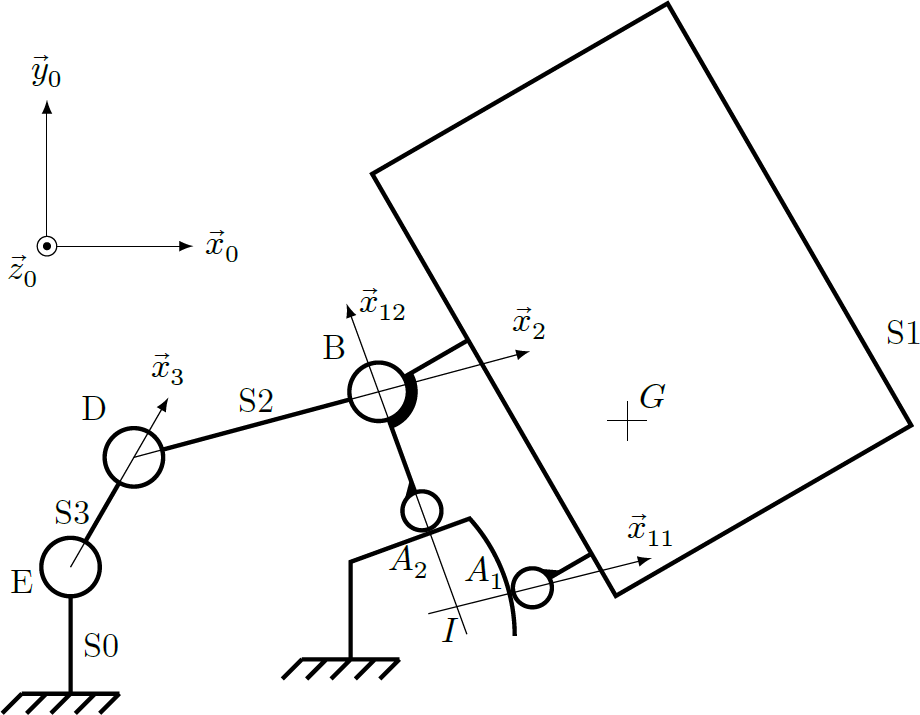
\includegraphics[width=\linewidth]{fig_04}
\end{marginfigure}

\begin{obj}
Suite à  l’appui  sur  le bouton d’arrêt d’urgence, le robot doit immédiatement s’immobiliser dans la position courante. On souhaite alors  vérifier  que  les  freins  équipant  le  robot  sont  suffisants  pour  assurer  sa  configuration 
d’équilibre dans le cas d’une charge maximale de \SI{50}{daN} (préhenseur + bidon de 40 litres) et 
qu’il ne faudra pas mettre des actionneurs en parallèle. 
\end{obj}

On se place dans la situation particulière définie figure suivante avec  $\alpha_2= -90\degres$ et $\alpha_3 = +90\degres$. 

On donne :
\begin{itemize}
\item $O_2O_3 = O_6O_7 = \SI{1250}{mm}$; 
\item $O_3O_{10} = O_8O_9 = \SI{1350}{mm}$; 
\item $O_2O_6 = O_3O_7 = O_3O_8 = O_9O_{10} = \SI{500}{mm}$ ; 
\item $\vect{P} = -500\vect{z_4}$.
\end{itemize}


\begin{marginfigure}
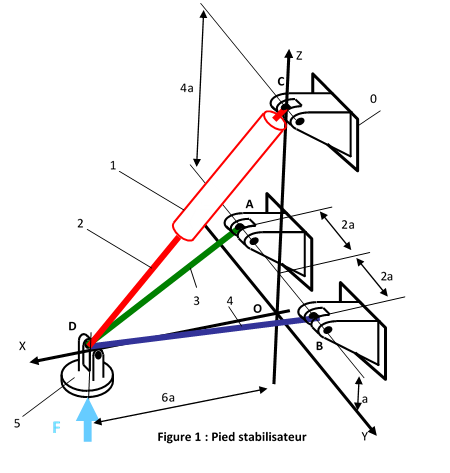
\includegraphics[width=\linewidth]{fig_02}
\end{marginfigure}

On admettra pour simplifier que le point $O_4$ est situé sur l’axe  $\vect{x_3}$ et que l’axe $\vect{z_4}$ passe par le 
point  $O_9$.  De  même,  les  poids  propres  des  pièces  seront  négligés  par  rapport  aux  autres 
actions. 

Les liaisons pivot sont supposées parfaites (pas de frottement). 

Les  couples de  freinage maxi $Mf_2$ et $Mf_3$ des  freins  associés  aux moteurs $M_2$ et $M_3$ sont de 
\SI{5}{mN} sur l’arbre moteur. On leur adjoint en série un réducteur de rapport 1/200. 



\question{Réaliser le graphe de structure du mécanisme.}
\ifprof
\begin{corrige}~\\

\end{corrige}
\else
\fi


\question{Déterminer les actions de la barre 8 sur le poignet 4 et du bras 3 sur le poignet 4.}
\ifprof
\begin{corrige}~\\

\end{corrige}
\else
\fi

\question{En isolant l’ensemble 3 et 4 et en considérant les informations fournies dans le tableau suivant, déterminer l’expression du moment $Mf_3$ correspondant à l’action
du frein sur la pièce 3 en $O_3$. }
\ifprof
\begin{corrige}~\\

\end{corrige}
\else
\fi

\begin{center}
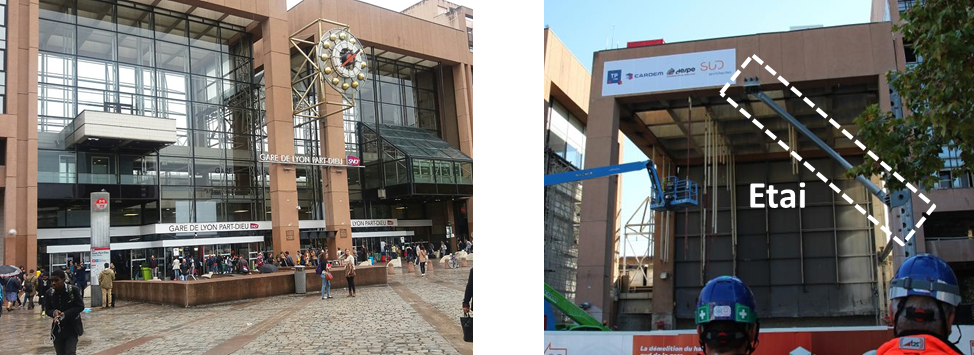
\includegraphics[width=\linewidth]{fig_03}
%\textit{}
\end{center}

Le dispositif de freinage ne permet qu’un couple maxi de \SI{5}{mN} sur l’axe moteur.

\question{Quel est alors le couple de freinage disponible en sortie du réducteur ?}
\ifprof
\begin{corrige}~\\

\end{corrige}
\else
\fi


\question{Le maintien du freinage est-il assuré ? }
\ifprof
\begin{corrige}~\\

\end{corrige}
\else
\fi
 
 On veut alors vérifier que le dispositif de freinage du moteur $M_2$ convient.

\question{En isolant la pièce 7, déterminer l’action de la barre 6 sur la pièce 7.}
\ifprof
\begin{corrige}~\\

\end{corrige}
\else
\fi
 

\question{En considérant l’ensemble 2, 3, 4, 7, 8, déterminer l’expression du moment $Mf_2$
correspondant à l’action du frein sur la pièce 2 en $O_2$. Calculer $Mf_2$. }
\ifprof
\begin{corrige}~\\

\end{corrige}
\else
\fi
 

\question{Le dispositif de freinage étant identique à celui de l’axe 3, le maintien du freinage
est-il assuré ?}
\ifprof
\begin{corrige}~\\

\end{corrige}
\else
\fi
 

\ifprof
\begin{center}
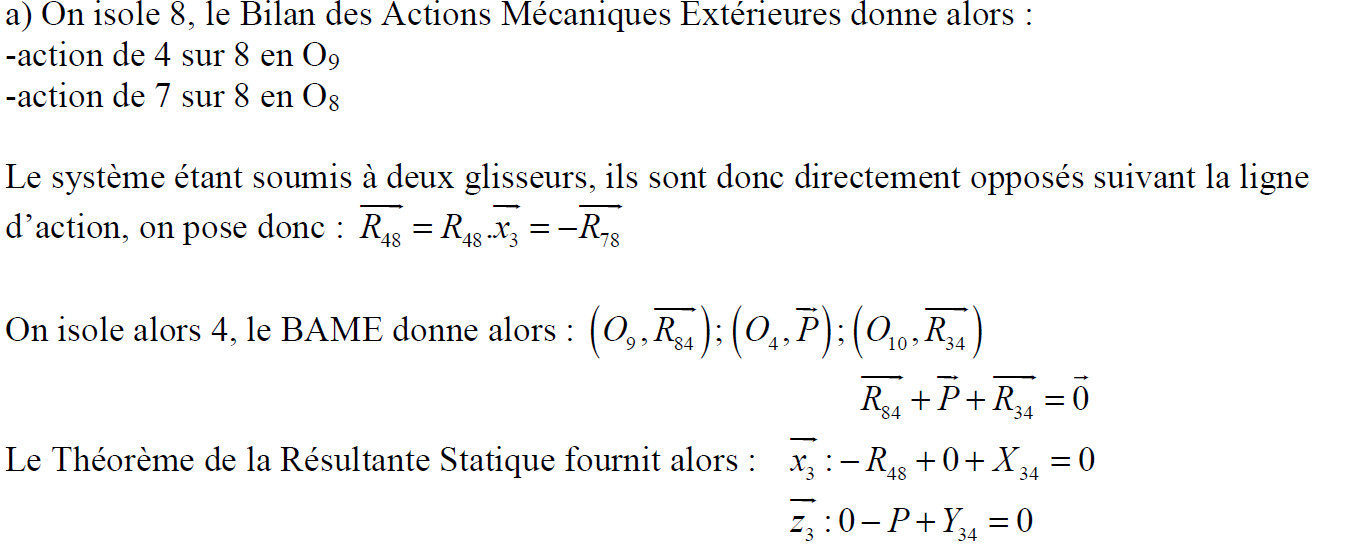
\includegraphics[width=\linewidth]{cor_01}
%\textit{}
\end{center}
\begin{center}
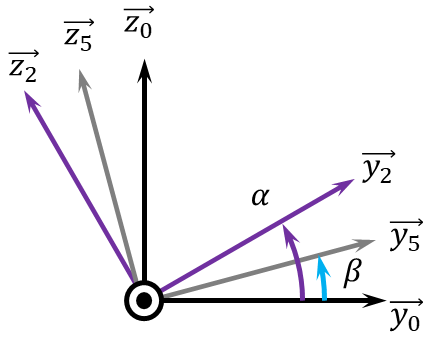
\includegraphics[width=\linewidth]{cor_02}
%\textit{}
\end{center}
\begin{center}
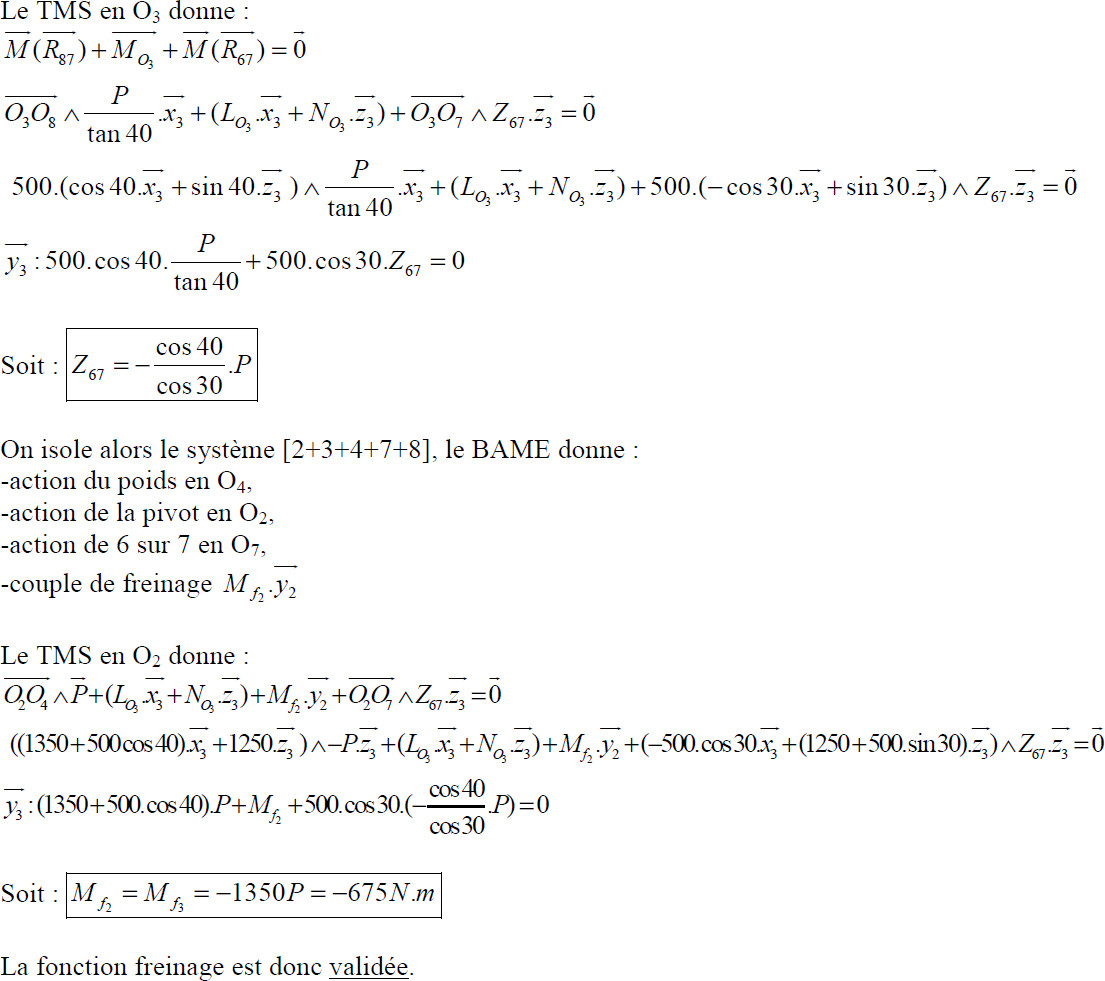
\includegraphics[width=\linewidth]{cor_03}
%\textit{}
\end{center}

\else\fi